\documentclass[11pt,a4paper]{article}
\usepackage[top=2.2cm,bottom=2.2cm,left=2.3cm,right=2.3cm]{geometry}
\usepackage[T1]{fontenc}
\usepackage{newtxtext,newtxmath}
\usepackage{microtype,amsmath,booktabs,array,tabularx,graphicx,xcolor,float,caption,enumitem,longtable,tikz,tcolorbox,cite,url}
\usepackage[colorlinks=true,linkcolor=blue!50!black,citecolor=blue!50!black,urlcolor=blue!50!black]{hyperref}
\usepackage{titlesec,fancyhdr}
\usetikzlibrary{arrows.meta,positioning}
\definecolor{navy}{HTML}{0B3D6B}
\titleformat{\section}{\Large\bfseries\color{navy}}{\thesection}{0.6em}{}
\titleformat{\subsection}{\large\bfseries\color{navy}}{\thesubsection}{0.6em}{}
\setlength{\parindent}{0pt}\setlength{\parskip}{5pt}
\newcolumntype{Y}{>{\raggedright\arraybackslash}X}
\pagestyle{fancy}\fancyhf{}\cfoot{\footnotesize LeakLens: the complete report in plain language \,|\, \thepage}\renewcommand{\headrulewidth}{0pt}
\captionsetup{font=small,labelfont=bf}
\newtcolorbox{key}[1][]{colback=navy!6,colframe=navy!60,boxrule=0.5pt,arc=2pt,left=6pt,right=6pt,top=4pt,bottom=4pt,#1}
\newtcolorbox{note}[1][]{colback=orange!8,colframe=orange!70!black,boxrule=0.5pt,arc=2pt,left=6pt,right=6pt,top=4pt,bottom=4pt,#1}
\newcommand{\code}[1]{\texttt{#1}}
\begin{document}
\begin{titlepage}
\centering\vspace*{2cm}
{\Huge\bfseries\color{navy} LeakLens}\\[6pt]
{\LARGE Water Leak Localization System}\\[1.3cm]
{\Large The Complete Project Report\\ in Plain Language}\\[1.2cm]
{\large What it is, how it works, how we test it, and what every number means}\\[1.8cm]
{\large\bfseries B.Tech Project, Semester 1}\\[3pt]
Indian Institute of Information Technology Kottayam\\[0.8cm]
\textbf{Guide:} Dr.\ Divya Sindhu Lekha\\[0.5cm]
Ashish Ranjan (2023BCS0027) \,\textbullet\, Nidamanuri Kedar Vaishnav (2023BCS0163)\\
Abhinandh Rajeev (2023BCS0074) \,\textbullet\, Kadthala Hrishith Reddy (2023BCS0168)\\[1.2cm]
October 2026\\[1.5cm]
\begin{minipage}{0.85\linewidth}\small
Every result in this report comes from computer simulation of water networks (EPANET through the WNTR tool). No real sensors or real utility data were used. The numbers show how the method behaves on three standard test networks; they are not a promise about performance in a real city.
\end{minipage}
\end{titlepage}

\tableofcontents
\newpage

\section{The project at a glance}
\begin{key}
\textbf{What problem does it solve?} A city's water pipes leak. Finding \emph{that} something is wrong is not enough: a pump stopping, a hydrant opening or a tank running low also change the water pressure. LeakLens tells these apart and, when it is a leak, points to \emph{where} it is.

\textbf{What does it do?} It simulates water networks on a computer, compares each situation with a normal day, follows the water to see whether any is disappearing, decides what kind of event it is, and ranks the places to look.

\textbf{How is it delivered?} A web dashboard (LeakLens) backed by a small server, so that a person can pick a situation, press one button and read a plain-language verdict.
\end{key}

\textbf{Headline results} (measured only on 139 test scenarios that the system never saw while learning):
\begin{center}\begin{tabular}{@{}lr@{}}\toprule
Question & Answer \\\midrule
Is the leak's exact node the first one the system lists? & \textbf{96.7\%} of 60 test leaks \\
Is the real leak among the first five nodes listed? & \textbf{98.3\%} \\
How often does a normal day trigger a false alarm? & \textbf{0.0\%} (a fixed 0.5 m alarm: 41.7\%) \\
How often is the \emph{kind} of event named correctly? & \textbf{82.7\%} (on scenarios it learned from: 95.6\%) \\
Time to analyse one scenario & about 22 milliseconds \\\bottomrule\end{tabular}\end{center}
The sections that follow explain every one of these, how it is measured, and where the system is weak.

\section{Why this matters}
Water utilities lose a large share of the treated water they produce to leaks and unmetered use, often called non-revenue water. The literature reports leakage from about 3\% to over 50\% depending on maintenance~\cite{sousa2026review}, and our presentation quotes about 40\% for developing countries. Leaks waste water and energy, damage roads and buildings and can let dirt into the pipes.

Finding leaks by walking the streets with listening equipment is slow. A pressure or flow sensor can show that something changed, but a pressure drop alone is ambiguous: a hot day, a pump failure or a leak can all lower the pressure. The practical question is therefore:

\begin{quote}\itshape When pressure and flow change in a water network, is it a leak or just a normal change in operation, and if it is a leak, which node is it?\end{quote}

Related research tests one network at a time, treats ``is there a leak?'' and ``where?'' as separate problems, or uses black-box models that are hard to explain~\cite{soldevila2021hybrid,sun2020leak,leonzio2026centrality,zhang2026aignn}. Our aim is an explainable pipeline that is tested on several networks and says \emph{why} it reached its answer.

\section{The idea in plain words}
Think of a bank account. Money comes in, customers spend some, and the rest stays. If money goes missing and no customer spent it, someone took it. A water node works the same way:

\begin{center}\textbf{water in $-$ water out $=$ water customers use $+$ water that leaks}\end{center}

If we know how much water the customers at each node really use (from smart meters), then any water that leaves a node and is not accounted for by a customer meter must be leaking. We call this \textbf{unaccounted flow}. A leak makes a large unaccounted flow at one node. A demand change does not, because the meters record it. A pump stopping or a tank changing alters the pressure across a wide area but loses no water.

That one idea, plus careful handling of sensor noise, does most of the work in LeakLens.

\section{The water networks}
We use three standard benchmark networks supplied with EPANET, the engineering standard for modelling water pipe networks. Each is a graph: junctions (where customers draw water) joined by pipes, with reservoirs (sources), tanks (storage) and pumps.
\begin{center}\small\begin{tabular}{@{}lcccc@{}}\toprule
Network & Junctions & Pumps & Tanks & Reservoirs \\\midrule
Net1 (small) & 9 & 1 & 1 & 1 \\
Net2 (medium) & 35 & 0 & 1 & 0 \\
Net3 (large benchmark) & 92 & 2 & 3 & 2 \\\bottomrule\end{tabular}\end{center}
Net2 has no reservoir or pump; one junction with negative demand acts as its supply.

\section{The scenarios}
A \textbf{scenario} is one 24-hour computer simulation of a network in which one thing (or a few things together) differs from the normal day. We built 617 scenarios on the three networks. For each we save, every hour, the pressure at every node, the flow in every pipe and the water actually delivered to customers at every node, together with the \emph{true answer} (what was changed and where) so that we can later check the system.
\begin{center}\small\begin{tabularx}{\linewidth}{@{}>{\bfseries}p{2.6cm}p{1.2cm}Y@{}}\toprule
Kind & Count & What is changed \\\midrule
Leak & 299 & A hole opens at one junction. Five sizes (tiny to burst), every junction, four start times, with and without sensor noise, and hidden behind another event (hydrant, demand surge, blocked pipe or pump outage). \\
Demand change & 60 & One node uses 1.5$\times$ or 0.5$\times$ as much; all nodes use 1.3$\times$ or 0.7$\times$; or a hydrant is opened for four hours. \\
Pump or reservoir & 54 & A pump is switched off for 2, 4 or 6 hours; or a reservoir level is raised or lowered by 2, 5 or 10 metres. \\
Tank change & 60 & A tank starts 10--90\% full, or is cut off from the network. \\
Blocked pipe & 48 & A busy pipe is closed, or is partly blocked. \\
Pipe ageing & 42 & All pipes become rougher (older, scaled pipes waste more pressure). \\
Normal day & 54 & Nothing changes; only random sensor errors, small or large, or none. \\\bottomrule\end{tabularx}\end{center}

\subsection{What each event does to the network}
\begin{itemize}[itemsep=3pt]
\item \textbf{Leak.} Water escapes through the hole. The amount grows with pressure: $Q=0.75\,A\sqrt{2gP}$ for a hole of area $A$ at pressure head $P$. Flow towards the leak rises and pressure falls around it, most at the leak. The loss is \emph{local} and \emph{unmetered}.
\item \textbf{Demand change.} Customers use more or less. Pressure falls where the use is heavy, much like a leak, but the extra flow is \emph{metered}.
\item \textbf{Pump or reservoir.} The places where water and pressure enter the network change. A pump switched off removes the energy it adds, so pressure falls over a wide area; a reservoir shifted by 5 m shifts the pressure of the whole network by about 5 m. No water is lost.
\item \textbf{Tank change.} A tank that starts low or is cut off changes how much it supplies; flow reroutes. No water is lost.
\item \textbf{Blocked pipe.} The pipe's flow is forced elsewhere. Pressure falls downstream and may rise upstream. No water is lost.
\item \textbf{Pipe ageing.} Rougher pipes lose more pressure for the same flow, slowly and widely. No water is lost.
\end{itemize}
\begin{figure}[H]\centering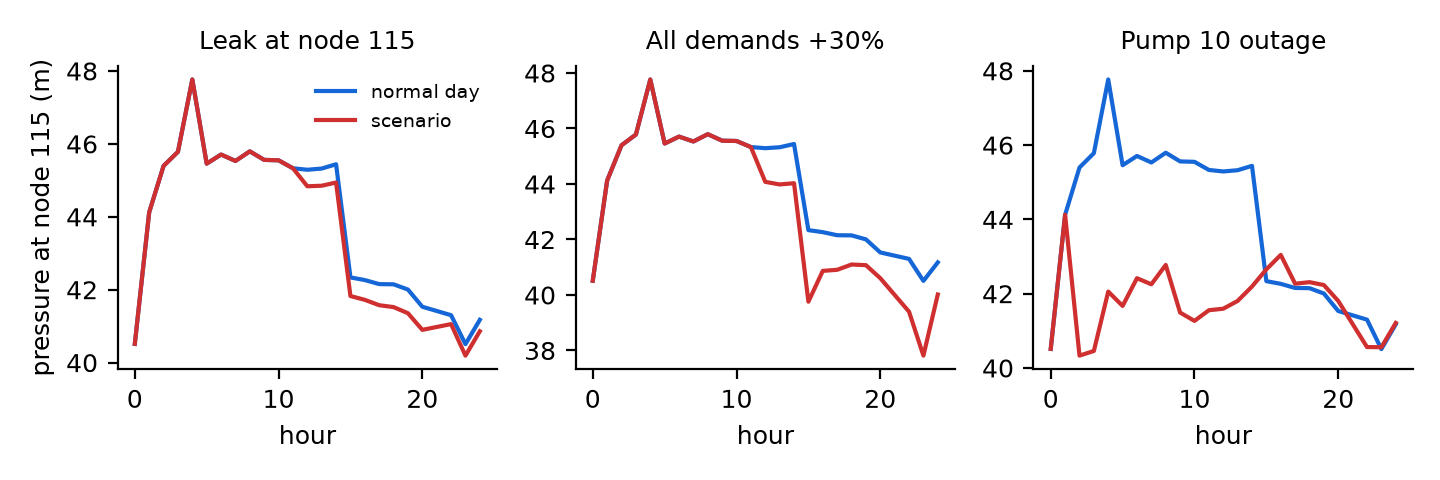
\includegraphics[width=\linewidth]{figures/fig_pressure.png}
\caption{Pressure at one Net3 node on a normal day (blue) and in three scenarios (red): a leak (steps down from noon), a demand surge (lower all day) and a pump outage (drops while the pump is off).}\end{figure}

\subsection{Sensor noise}
Real sensors are not perfect. In ``noisy'' scenarios we add random errors (pressure $\pm0.05$ or $0.2$ m; flows and demands $0.5\%$ or $2\%$). The normal-day reference is kept clean: it stands for what the hydraulic model expects.

\section{How the system analyses one scenario}
\begin{center}
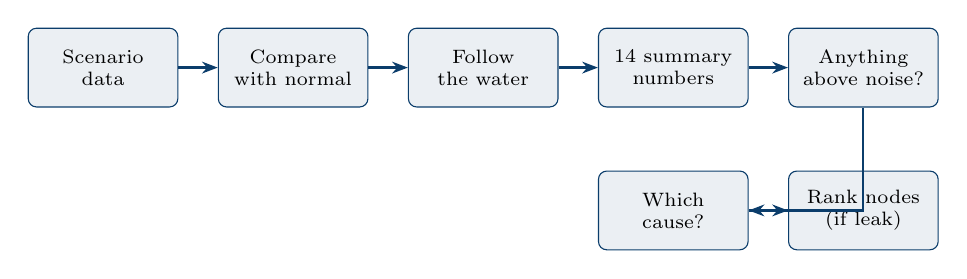
\begin{tikzpicture}[node distance=5mm,
 box/.style={draw=navy,fill=navy!8,rounded corners=3pt,minimum width=1.9cm,minimum height=1.0cm,align=center,font=\scriptsize},
 arr/.style={-{Stealth[length=2mm]},thick,navy}]
\node[box](a){Scenario\\data};
\node[box,right=of a](b){Compare\\with normal};
\node[box,right=of b](c){Follow\\the water};
\node[box,right=of c](d){14 summary\\numbers};
\node[box,right=of d](e){Anything\\above noise?};
\node[box,below=8mm of d](f){Which\\cause?};
\node[box,right=of f](g){Rank nodes\\(if leak)};
\draw[arr](a)--(b);\draw[arr](b)--(c);\draw[arr](c)--(d);\draw[arr](d)--(e);\draw[arr](e.south)|-(f.east);\draw[arr](f)--(g);
\end{tikzpicture}
\end{center}

\textbf{Step 1: compare with the normal day.} For every node and hour we subtract the scenario's pressure from the normal day's. A drop only counts if it stays above the noise threshold for two hours in a row, so one odd reading cannot trigger anything.

\textbf{Step 2: learn what noise looks like.} Each network has 18 normal runs that contain only sensor noise; the learning (training) ones are used to measure how big the noise normally is. The pressure threshold is four times that spread, about 0.5--0.6 m. A fixed 0.5 m alarm ignores this and raises many false alarms (41.7\% of normal test days).

\textbf{Step 3: follow the water.} For each node we work out how much water went in minus out, subtract the change in customer use, and what remains is the \emph{unaccounted flow}, which is the leak flow.
\begin{figure}[H]\centering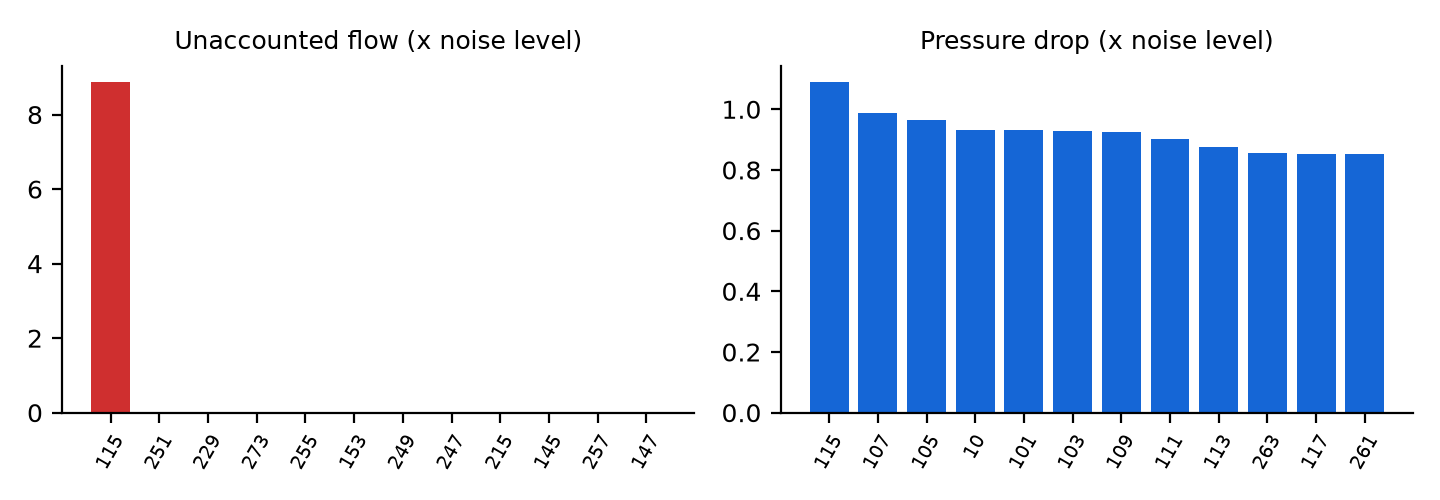
\includegraphics[width=\linewidth]{figures/fig_signals.png}
\caption{A leak at one Net3 node. Left: unaccounted flow is large at the leak node and nearly zero elsewhere. Right: the pressure drop is high at the leak but also at its neighbours, so pressure alone is blurrier.}\end{figure}

\textbf{Step 4: fourteen summary numbers.} Each scenario is boiled down to 14 numbers, for example: the share of junctions that lost pressure, the biggest unaccounted flow, how much flow a pump lost, how much the reservoir supply and the tanks changed. All are measured in units of the noise level or as a share of total demand, so they are comparable between networks.

\textbf{Step 5: is anything above noise?} If every number is within noise, the answer is \emph{normal day} and the analysis stops. This is why normal days do not cause false alarms. It also means leaks smaller than the noise cannot be seen.

\textbf{Step 6: which cause?} A \emph{random forest} (300 small decision trees that vote) looks at the 14 numbers and gives a probability for each of: normal, leak, demand change, pump/reservoir, tank, blocked pipe, ageing. The highest probability is the verdict; that probability is the confidence (High from 85\%, Medium from 60\%, otherwise Low). This is the only step that is \emph{learned} from data; everything else is calculation.

\textbf{Step 7: rank the nodes (leaks only).} Each junction gets a score
\[\text{score}=A+0.3\,D,\]
where $A$ is its unaccounted flow and $D$ its pressure drop, each scaled so that the largest in the network is 1. The unaccounted flow is the main signal; the pressure drop is a backup. Nodes are sorted by score: the first is the system's best guess, the next ones are where to look if it is wrong. The ranking is a fixed formula, not a trained model.

\subsection{A worked example}
In Net3 a leak is opened at node 115. The leak node has the largest unaccounted flow ($A=1.00$) and the largest pressure drop ($D=1.00$), so its score is $1.00+0.3\times1.00=1.30$. Its neighbours, nodes 107 and 105, have almost no unaccounted flow ($A\approx0$) but a large pressure drop ($D\approx0.9$), so they score only about $0.27$. Node 115 is clearly first. This is a ``Top-1 success'': the true leak is the first node on the list, zero pipes away.

\section{How the system is trained and tested}
\begin{key}
If you test a system on the same examples it learned from, it can score perfectly just by remembering them, and you learn nothing about new situations. So we keep some scenarios completely aside.
\end{key}
All 617 scenarios were split once, with a fixed random seed, into about \textbf{80\% for learning} and \textbf{20\% for testing}.
\begin{center}\small\begin{tabular}{@{}lrrr@{}}\toprule
Kind & All & Learning (train) & Testing (test) \\\midrule
Normal day & 54 & 42 & 12 \\
Leak & 299 & 232 & 67 \\
Demand change & 60 & 48 & 12 \\
Pump / reservoir & 54 & 42 & 12 \\
Tank change & 60 & 48 & 12 \\
Blocked pipe & 48 & 36 & 12 \\
Pipe ageing & 42 & 30 & 12 \\
\midrule
Total & 617 & 478 & 139 \\
\bottomrule\end{tabular}\end{center}
\begin{itemize}[itemsep=3pt]
\item \textbf{Learned only from the training scenarios:} the noise thresholds and the random forest.
\item \textbf{Measured only on the test scenarios:} every accuracy, false-alarm and Top-$k$ figure in this report. The system never saw these while learning.
\item \textbf{Near-copies stay together.} All leaks at the same junction (every size, start time, noise level and ``hidden behind'' variant) go to the same side, and a scenario goes with its sensor-noise twin. Otherwise a test scenario could be almost identical to a training one, and the test would be too easy.
\item \textbf{Fair mix.} Each network and each kind of event is split about 80/20.
\item The dashboard tags every scenario \emph{Unseen test} or \emph{Training}, and shows unseen ones by default.
\end{itemize}
The leak-ranking formula (weight 0.3, no neighbour smoothing) and the cut-offs in step 5 were chosen during development while looking at all the scenarios, before the split existed. They were not re-tuned afterwards. The test set is small, so each percentage has a wide margin of error.

\section{What the metrics mean}
This section explains every number used later, in plain words, with a small example. Think of the system's job in three parts: noticing a problem (detection), naming it (classification) and finding it (localization).

\subsection{Detection: is something wrong?}
Here a scenario is ``positive'' if any abnormal event happened (leak, demand change, pump, tank, blockage, ageing) and ``negative'' if it is a normal day. Comparing the system's call with the truth gives four counts:
\begin{center}\small\begin{tabular}{@{}lcc@{}}\toprule
 & System says problem & System says normal \\\midrule
Truth: problem & true positive (TP) & false negative (FN, a miss) \\
Truth: normal day & false positive (FP, false alarm) & true negative (TN) \\\bottomrule\end{tabular}\end{center}
\begin{itemize}[itemsep=3pt]
\item \textbf{Precision} $=\frac{TP}{TP+FP}$. When the system raises an alarm, how often is it real? 100\% means no false alarms.
\item \textbf{Recall} $=\frac{TP}{TP+FN}$. Of the real problems, how many did it catch? 100\% means none missed.
\item \textbf{F1 score} $=\frac{2\cdot\text{precision}\cdot\text{recall}}{\text{precision}+\text{recall}}$. One number that is high only when both precision and recall are high.
\item \textbf{False-alarm rate} $=\frac{FP}{FP+TN}$. Of the normal days, how many wrongly raise an alarm?
\end{itemize}
\textit{Example from our test.} For the full system: $TP=119$, $FP=0$, $FN=8$, $TN=12$. So precision $=119/(119+0)=$ 100.0\%, recall $=119/(119+8)=$ 93.7\%, F1 $=$ 96.7\%, false-alarm rate $=0/(0+12)=$ 0.0\% (on 12 normal test days).

\subsection{Classification: what kind of event?}
\begin{itemize}[itemsep=3pt]
\item \textbf{Accuracy} $=$ correct answers $/$ all test scenarios. Easy to read but it can hide weak spots in small classes.
\item \textbf{Per-class precision, recall and F1.} The same three ideas as above, worked out separately for each kind of event. For ``leak'': precision is how often a ``leak'' verdict is really a leak; recall is how many real leaks get a ``leak'' verdict.
\item \textbf{Macro-F1} $=$ the plain average of the per-class F1 scores. Every kind counts equally, so a weak small class pulls it down.
\item \textbf{Confusion matrix.} A table: each row is the true kind, each column what the system said. A perfect system has numbers only on the diagonal.
\item \textbf{Train accuracy versus test accuracy.} Accuracy on the scenarios it learned from versus on unseen ones. A big gap means the model partly memorises.
\item \textbf{Leave-one-network-out.} Train on two networks, then test on the third network's test scenarios. It shows whether the system works on a network it has never seen.
\end{itemize}

\subsection{Localization: where is the leak?}
\begin{itemize}[itemsep=3pt]
\item \textbf{Rank.} Position of the true leak node in the system's sorted list (1 means first).
\item \textbf{Top-1 accuracy} $=\frac1N\sum\mathbf 1[\text{rank}=1]$: the share of leaks whose exact node is first. \textbf{Top-3} and \textbf{Top-5}: the true node is within the first 3 or 5.
\item \textbf{Pipe hops (error).} The number of pipes between the system's first guess and the true node. 0 is exact; 1 is the next junction along the pipe. We report the average.
\item \textbf{Within 1 hop.} Share of leaks where the first guess is the exact node or its direct neighbour.
\item \textbf{Error in metres.} The length of pipe on the shortest path between guess and truth.
\item \textbf{End-to-end.} Counts a leak as a success only if the system both called it a leak \emph{and} put the right node first.
\item \textbf{Inference time.} How long one analysis takes.
\end{itemize}
\textit{Example.} Over 60 test leaks, the exact node came first 58 times: Top-1 $=58/60=$ 96.7\%. The first version managed 35 of 60 (58.3\%). With only 60 leaks, one miss changes the percentage by about 1.7 points.

\section{Results}
\subsection{Detection}
\begin{center}\small\begin{tabular}{@{}lcccc@{}}\toprule
Method & Precision & Recall & F1 & False alarms \\\midrule
Fixed 0.5 m alarm (first version) & 95.7\% & 87.4\% & 91.4\% & 41.7\% \\
Learned pressure threshold & 100.0\% & 77.2\% & 87.1\% & 0.0\% \\
Full system (detector + cause model) & 100.0\% & 93.7\% & 96.7\% & 0.0\% \\
\bottomrule\end{tabular}\end{center}
The fixed 0.5 m alarm catches most problems but raises a false alarm on 41.7\% of normal days, because it ignores sensor noise. A threshold learned from each network's own normal runs, plus the ``anything above noise?'' check, raises none on the test days, while still catching 93.7\% of real problems.

\subsection{Which kind of event?}
Accuracy on unseen test scenarios: \textbf{82.7\%} (on the training scenarios: 95.6\%). Macro-F1: 76.4\%. Of the leaks, 89.6\% were named as leaks. All seven that were not are leaks at Net3 node 601, a pump-outlet node we exclude as unreliable (its pressure swings wildly for tiny changes); every other test leak was named a leak. Only 1.4\% of non-leaks were wrongly called a leak.
\begin{center}\small\begin{tabular}{@{}lcccc@{}}\toprule
Kind & Precision & Recall & F1 & Test scenarios \\\midrule
Normal day & 60.0\% & 100.0\% & 75.0\% & 12 \\
Leak & 98.4\% & 89.6\% & 93.8\% & 67 \\
Demand change & 100.0\% & 100.0\% & 100.0\% & 12 \\
Pump / reservoir & 66.7\% & 66.7\% & 66.7\% & 12 \\
Tank change & 57.1\% & 66.7\% & 61.5\% & 12 \\
Blocked pipe & 100.0\% & 75.0\% & 85.7\% & 12 \\
Pipe ageing & 54.5\% & 50.0\% & 52.2\% & 12 \\
\bottomrule\end{tabular}\end{center}
Confusion matrix on the test scenarios (rows = truth, columns = system's answer; a dot means zero):
\begin{center}\small\begin{tabular}{@{}l*{7}{r}@{}}\toprule
 & Normal & Leak & Demand & Pump & Tank & Blocked & Ageing \\\midrule
Normal day & 12 & . & . & . & . & . & . \\
Leak & 6 & 60 & . & . & 1 & . & . \\
Demand change & . & . & 12 & . & . & . & . \\
Pump / reservoir & 2 & . & . & 8 & 2 & . & . \\
Tank change & . & . & . & . & 8 & . & 4 \\
Blocked pipe & . & 1 & . & . & 1 & 9 & 1 \\
Pipe ageing & . & . & . & 4 & 2 & . & 6 \\
\bottomrule\end{tabular}\end{center}
\begin{figure}[H]\centering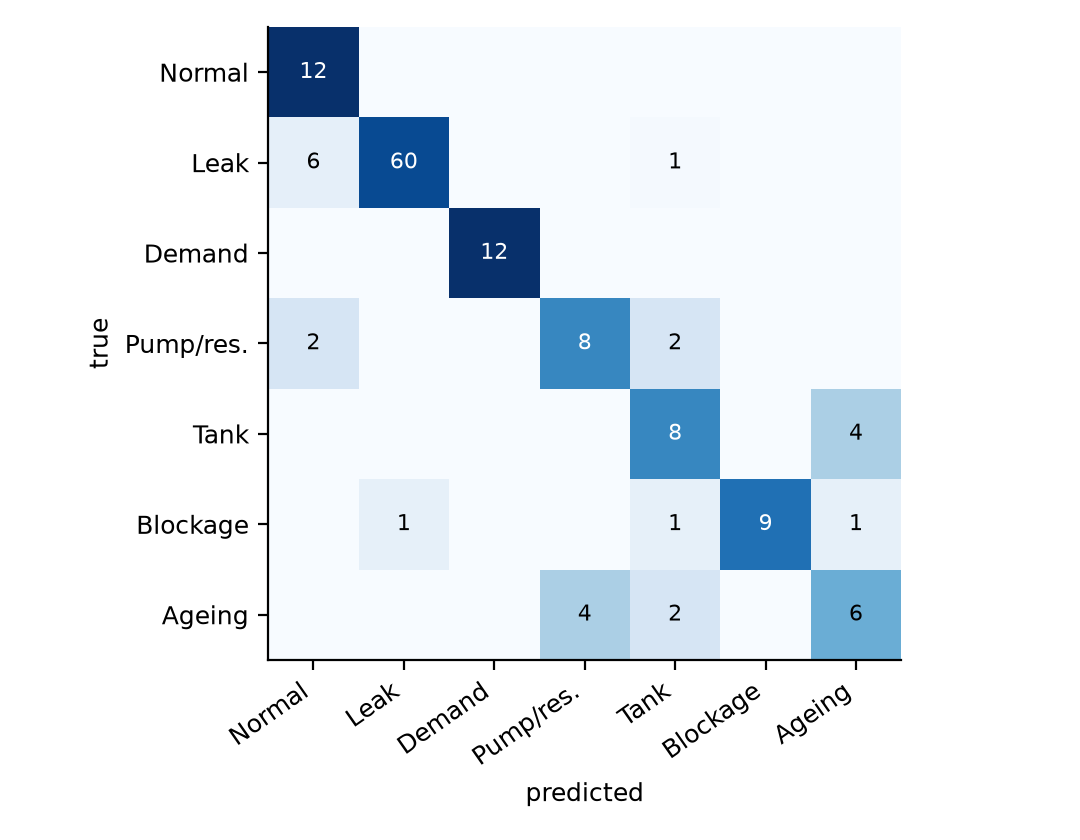
\includegraphics[width=0.55\linewidth]{figures/fig_confusion.png}\caption{The same matrix as a picture.}\end{figure}
\textbf{Reading it:} leaks and demand changes are recognised reliably. Pump, tank, blockage and ageing are sometimes mistaken for each other because each makes pressure fall across a wide area without losing water; some small events are reported as normal because they stay within the sensor noise.

\subsection{Where is the leak?}
\begin{center}\small\begin{tabular}{@{}lccccc@{}}\toprule
Method (60 test leaks) & Top-1 & Top-3 & Top-5 & Avg.\ hops & Within 1 hop \\\midrule
First version (pressure + 50 $\times$ flow) & 58.3\% & 70.0\% & 71.7\% & 3.35 & 58.3\% \\
\textbf{Final method} & 96.7\% & 98.3\% & 98.3\% & 0.13 & 96.7\% \\
Final + neighbour smoothing & 96.7\% & 98.3\% & 98.3\% & 0.13 & 96.7\% \\
Final, without demand meters & 93.3\% & 98.3\% & 98.3\% & 0.72 & 93.3\% \\
Pressure only & 60.0\% & 70.0\% & 70.0\% & 3.05 & 61.7\% \\
Pressure only + smoothing & 50.0\% & 63.3\% & 65.0\% & 3.18 & 58.3\% \\
\bottomrule\end{tabular}\end{center}
\begin{figure}[H]\centering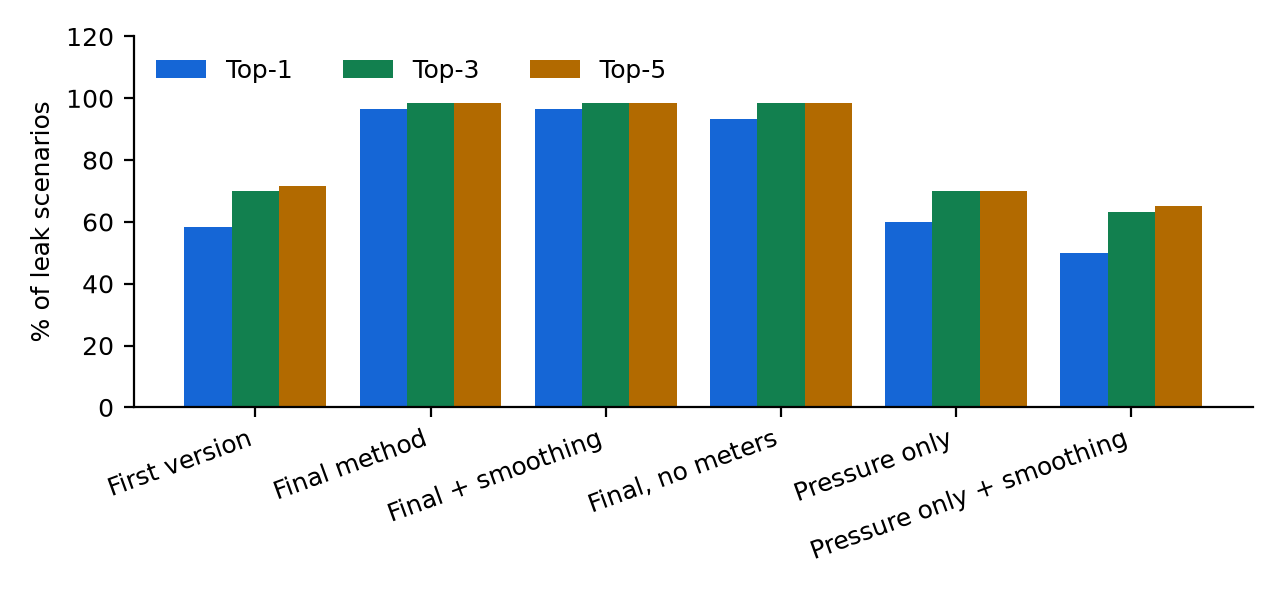
\includegraphics[width=0.85\linewidth]{figures/fig_localization.png}\caption{Localization accuracy of each method on the test leaks.}\end{figure}
\begin{itemize}[itemsep=3pt]
\item \textbf{Unaccounted flow is what works.} Using it lifts Top-1 from 58.3\% to 96.7\%. The final method is on average 0.13 pipes away (about 60 m) from the true node; 96.7\% of leaks are found at the node or its neighbour. End-to-end success is 96.7\%.
\item \textbf{Without demand meters} Top-1 is 93.3\%: a demand change at another node can look like a small leak.
\item \textbf{Pressure alone} reaches only 60.0\%, because the pressure drop spreads to neighbouring nodes.
\item \textbf{Smoothing the scores over neighbours} gave 96.7\%, no improvement, so it is not used. Network distance is used instead to measure the error and to define the search region.
\end{itemize}

\subsection{By type of leak}
\begin{center}\small\begin{tabular}{@{}lccc@{}}\toprule
Group (test leaks) & Leaks & Top-1 & Top-5 \\\midrule
Leak hidden behind another event & 10 & 100.0\% & 100.0\% \\
Leak with sensor noise & 4 & 100.0\% & 100.0\% \\
Leak size variations & 20 & 90.0\% & 95.0\% \\
Leak start time variations & 4 & 100.0\% & 100.0\% \\
Leak at a junction (clean data) & 22 & 100.0\% & 100.0\% \\
\midrule
Dead End & 17 & 100.0\% & 100.0\% \\
Hub & 1 & 100.0\% & 100.0\% \\
Inline & 42 & 95.2\% & 97.6\% \\
NET1 & 11 & 100.0\% & 100.0\% \\
NET2 & 26 & 92.3\% & 96.2\% \\
NET3 & 23 & 100.0\% & 100.0\% \\
\bottomrule\end{tabular}\end{center}
Leaks hidden behind another event are still found, because a hydrant or demand surge is metered and cancels out of the unaccounted flow. Small groups mean small differences should not be over-read.

\subsection{Leak size}
\begin{center}\small\begin{tabular}{@{}cccccc@{}}\toprule
Hole area (m$^2$) & Test leaks & Noticed by pressure & Called a leak & Exact node (Top-1) \\\midrule
0.0001 & 4 & 75.0\% & 100.0\% & 100.0\% \\
0.0003 & 4 & 100.0\% & 100.0\% & 100.0\% \\
0.001 & 4 & 100.0\% & 100.0\% & 100.0\% \\
0.003 & 4 & 100.0\% & 100.0\% & 100.0\% \\
0.01 & 4 & 100.0\% & 100.0\% & 50.0\% \\
\bottomrule\end{tabular}\end{center}
\begin{figure}[H]\centering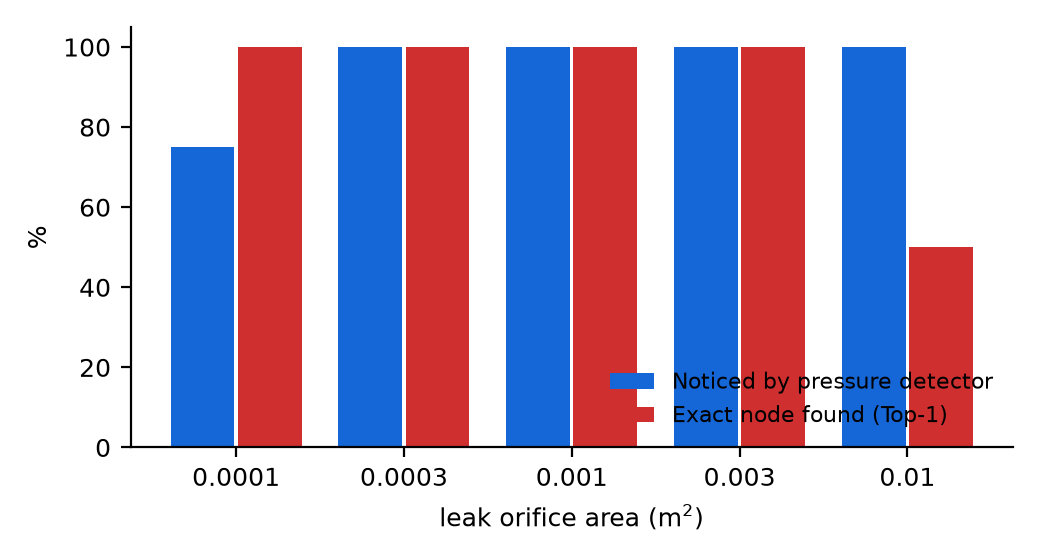
\includegraphics[width=0.6\linewidth]{figures/fig_size.png}\caption{Detection and exact-node success by leak size.}\end{figure}
Very small leaks sit close to the sensor noise; some are not noticed. The biggest leak lowers pressure across the whole network, so its exact node is the hardest to pick. There are only four test leaks per size, so this is indicative.

\subsection{A network the system has never seen}
Train on the training scenarios of two networks, test on the third network's test scenarios:
\begin{center}\small\begin{tabular}{@{}lccccc@{}}\toprule
Unseen network & Test scenarios & Overall accuracy & Leak recall & Leak precision & Accuracy without meters \\\midrule
NET1 & 33 & 48.5\% & 100.0\% & 100.0\% & 45.5\% \\
NET2 & 44 & 81.8\% & 92.3\% & 100.0\% & 75.0\% \\
NET3 & 62 & 54.8\% & 73.3\% & 100.0\% & 14.5\% \\
\bottomrule\end{tabular}\end{center}
Leaks mostly carry over to a new network. Telling pump, tank, blockage and ageing apart does not carry over well, and without demand meters the result on Net3 collapses to 14.5\%. This is the most important thing to improve in Semester 2.

\subsection{Training versus test}
Cause accuracy: \textbf{95.6\%} on training scenarios, \textbf{82.7\%} on test scenarios. Leak Top-1: \textbf{97.8\%} on training leaks, \textbf{96.7\%} on test leaks. The cause model shows a gap (it partly memorises); the ranking shows almost none, because it is a fixed formula that never trained.

\section{The software}
\subsection{Backend}
A FastAPI server runs the analysis and serves data to the dashboard. At start-up it creates an \textbf{SQLite} database and rebuilds a table of all scenarios from the saved files, including the Unseen test / Training tag, so the dashboard always lists exactly what exists.
\begin{center}\small\begin{tabularx}{\linewidth}{@{}>{\ttfamily}p{5.0cm}Y@{}}\toprule
Endpoint & What it returns \\\midrule
GET /api/networks & the three networks and how many scenarios each has \\
GET /api/scenarios?network= & the scenario list with details (kind, node, size, noise, test or training) \\
GET /api/network?network= & node positions and pipes for the map \\
GET /api/analyze/\{scenario\} & the verdict, probabilities, ranked nodes, search region, affected nodes, per-node and per-pipe numbers, and the true answer \\
GET /api/evaluation & the saved test results \\\bottomrule\end{tabularx}\end{center}

\subsection{Dashboard}
\begin{figure}[H]\centering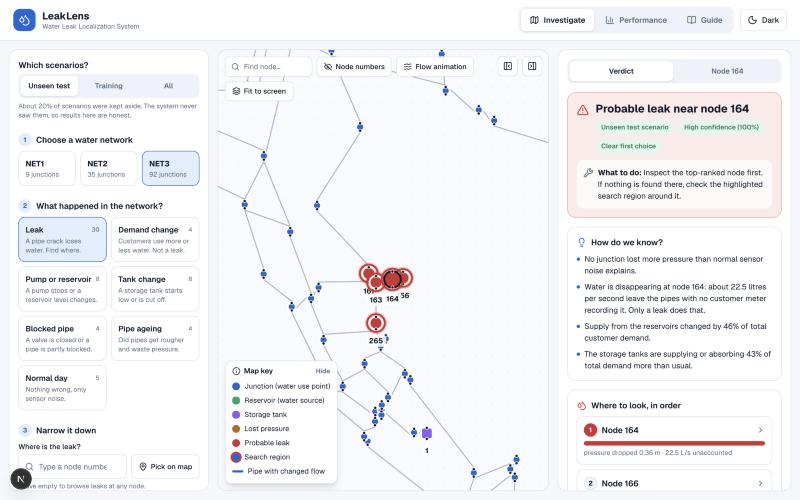
\includegraphics[width=0.98\linewidth]{figures/ui_light_leak.jpg}\caption{Light theme. Left: choose a situation. Centre: the network map. Right: the verdict, the reasons and the nodes to inspect, with an \emph{Unseen test} tag.}\end{figure}
The design goal was that a non-specialist can use it without reading a manual:
\begin{itemize}[itemsep=3pt]
\item \textbf{Guided choice, not a giant list.} Step 1 network, step 2 what happened (seven cards), step 3 narrow down: for leaks, type a node number or press \emph{Pick on map}, then choose a size and conditions. A counter shows how many scenarios match; \emph{Surprise me} and next/previous arrows replace scrolling.
\item \textbf{One-click examples} on the welcome panel.
\item \textbf{Plain-language verdict:} a headline, a confidence label, a \emph{What to do} line, and reasons written from the measurements (for example, ``22 litres per second leave the pipes with no customer meter recording it''). Technical details are folded away.
\item \textbf{Explained words:} dotted-underline terms show a definition on hover or tap; a Guide tab lists them.
\item \textbf{Honest testing built in:} the Unseen test / Training tag on every scenario and a warning if you analyse a training scenario.
\item \textbf{Light and dark themes,} keyboard-friendly controls, a phone layout, and collapsible side panels.
\item \textbf{Performance tab:} the results of this report in plain language.
\end{itemize}
\begin{figure}[H]\centering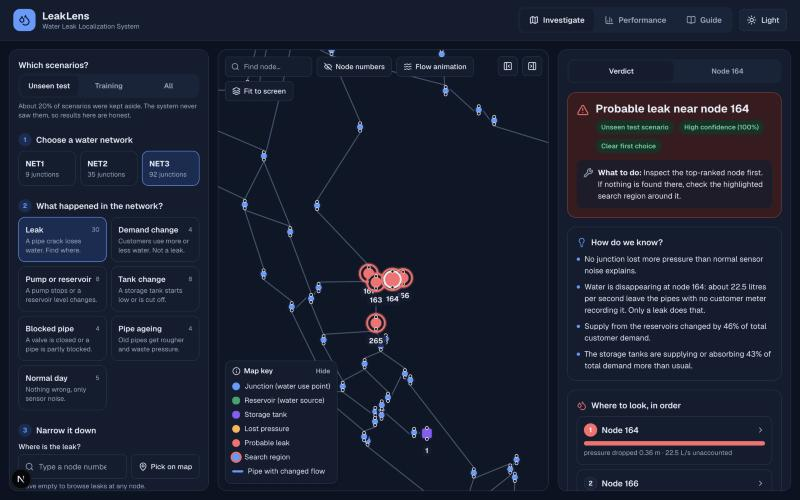
\includegraphics[width=0.98\linewidth]{figures/ui_dark_leak.jpg}\caption{Dark theme, a leak found at the first node of the list, with its search region around it.}\end{figure}
\begin{figure}[H]\centering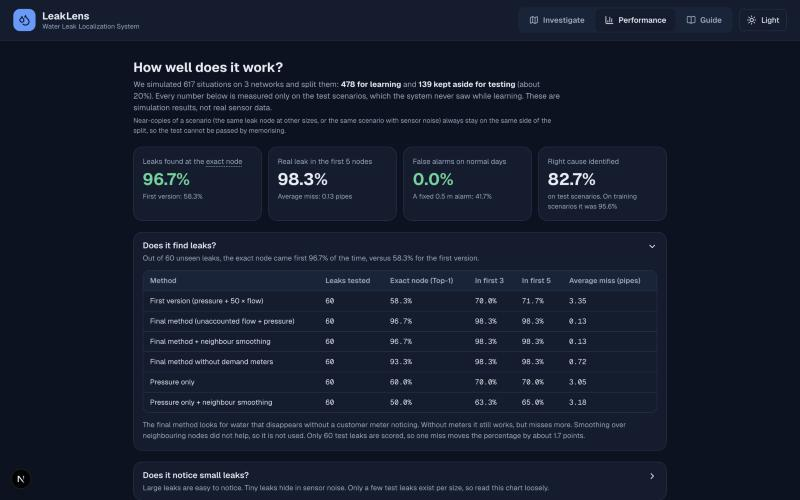
\includegraphics[width=0.98\linewidth]{figures/ui_performance.jpg}\caption{The Performance tab: test results with the learning/testing split stated at the top.}\end{figure}

\subsection{What the screen says, and where it comes from}
The sentences under ``How do we know?'' are not written by a language model. They are fixed templates that appear when one of the 14 numbers passes a limit, with the real values filled in. For example, ``a pump lost 100\% of its flow'' appears when the pump-flow number is above 0.5; ``water is disappearing at node X'' appears when the unaccounted flow is above the noise level.

\section{How to run it}
\begin{enumerate}[itemsep=2pt]
\item \code{python simulation/build\_scenarios.py} builds the scenario list.
\item \code{python simulation/generate\_dataset.py --force} runs the simulations (about 30 seconds).
\item \code{python ml\_pipeline/train.py} trains the cause model on the training scenarios.
\item \code{python ml\_pipeline/evaluate.py} measures everything on the test scenarios.
\item \code{cd backend \&\& uvicorn main:app --port 8000} starts the server.
\item \code{cd frontend \&\& npm run dev} starts the dashboard at \code{http://localhost:3000}.
\end{enumerate}

\section{Honest limitations}
\begin{note}
These matter when you present or rely on the results.
\end{note}
\begin{itemize}[itemsep=3pt]
\item \textbf{Simulation only.} Real networks have real noise, errors in the model and surprises we did not simulate.
\item \textbf{Small test set.} 139 test scenarios, 60 scored leaks and 12 normal days. One miss moves a percentage by about 1.7 points, and the split was made once.
\item \textbf{Settings chosen before the split.} The ranking weight and the cut-offs used all scenarios and were not re-tuned.
\item \textbf{Demand meters are assumed.} Real utilities usually meter an area, not each node. Without per-node meters leak ranking and cause accuracy drop.
\item \textbf{Small leaks are missed} when everything stays within the sensor noise.
\item \textbf{The biggest leaks are hard to pinpoint} because they lower pressure everywhere.
\item \textbf{Causes do not transfer well to unseen networks.} Pump, tank, blockage and ageing events are confused, most in the very small Net1.
\item \textbf{Gap between training and test accuracy} (95.6\% versus 82.7\%): the cause model partly memorises.
\item \textbf{Excluded readings:} two Net3 nodes next to a pump outlet and one hour of pump switching were ignored because they swing wildly for tiny changes. Pump speed changes were not simulated (the simulator does not support them), and some blockage cases did not converge and were dropped.
\end{itemize}

\section{What comes next (Semester 2)}
Missing and sparse sensors (using graph methods to choose where to put sensors~\cite{leonzio2026centrality}); estimating demand where nodal meters do not exist; several leaks at once; cause classification that carries over to new networks, including graph or algorithm-informed models~\cite{zhang2026aignn} compared against this interpretable baseline; a larger, repeatedly re-split test; and validation on public benchmark data or real utility data.

\section{Glossary}
\begin{center}\small\begin{tabularx}{\linewidth}{@{}>{\bfseries}p{3.2cm}Y@{}}\toprule
Term & Meaning \\\midrule
Baseline / normal day & The simulated day with nothing wrong, used as the reference. \\
Junction, reservoir, tank, pump & Water use point; water source; storage; machine that adds pressure. \\
Pressure (m) & How hard water pushes in a pipe, as metres of water column. \\
Flow (L/s) & Litres of water passing a point each second. \\
Demand & Water customers actually draw at a node. \\
Demand meter & A meter reporting customer use at a node. \\
Unaccounted flow & Water leaving a node that no meter records: the leak flow. \\
Sensor noise & Small random errors in readings. \\
Scenario & One simulated 24-hour situation with a known true answer. \\
Training / test scenarios & Scenarios the system learns from / keeps aside to be tested on. \\
Random forest & Many small decision trees that vote on the answer. \\
Precision, recall, F1 & How often an alarm is real; how many real events are caught; a combined score. \\
False-alarm rate & Share of normal days that trigger an alarm. \\
Confusion matrix & Table of true kind versus the system's answer. \\
Top-1 / Top-5 & The true leak is first / within the first five nodes. \\
Pipe hop & One pipe between two nodes; used to count how far a guess is from the truth. \\
Search region & The predicted node and its direct neighbours. \\
Leave-one-network-out & Training on two networks and testing on the third. \\\bottomrule\end{tabularx}\end{center}

\begingroup\footnotesize
\begin{thebibliography}{9}
\raggedright
\bibitem{sousa2026review} A.~L. Sousa, A.~F. Brochado, E. Rocha, and A. Andrade-Campos, ``A state-of-the-art review of scientific, industrial, and commercial developments in water leakage management for water supply systems,'' \emph{Water Research}, vol.~299, 125853, 2026.
\bibitem{soldevila2021hybrid} A. Soldevila, G. Boracchi, M. Roveri, S. Tornil-Sin, and V. Puig, ``Leak detection and localization in water distribution networks by combining expert knowledge and data-driven models,'' \emph{Neural Comput.\ Appl.}, vol.~34, no.~6, pp.~4759--4779, 2022.
\bibitem{sun2020leak} C. Sun, B. Parellada, V. Puig, and G. Cembrano, ``Leak localization in water distribution networks using pressure and data-driven classifier approach,'' \emph{Water}, vol.~12, no.~1, 54, 2020.
\bibitem{leonzio2026centrality} D.~U. Leonzio, T. Cattai, P. Bestagini, S. Colonnese, and S. Tubaro, ``Centrality-guided node selection for efficient water leak detection,'' \emph{IEEE Access}, vol.~14, pp.~24432--24446, 2026.
\bibitem{zhang2026aignn} Z. Zhang and O. Fink, ``Algorithm-informed graph neural networks for leakage detection and localization in water distribution networks,'' \emph{Reliab.\ Eng.\ Syst.\ Saf.}, vol.~265, 111494, 2026.
\end{thebibliography}
\endgroup
\end{document}
